\section{Data, Features, Models}

This section will mainly focus on data, features, and models.
As has been mentioned in the previous section the first key element
of machine learning is \emph{data}. Then, by processing these data,
the second main key will be extracted, the so-called \emph{features},
which are the most relevant part of the data that will be used for
learning. Finally, based on the features extracted previously, it will
be possible to build the so-called \emph{models} that will represent the
summary of the knowledge acquired through the learning process and will
be used to perform some actions.

\subsection{Learning Process}

Based on the results provided in the previous section, it is time to
introduce a more complete description of the machine learning pipeline,
as illustrated in the image below:

\vspace{5mm}

\begin{figure}[h]
      \centering
      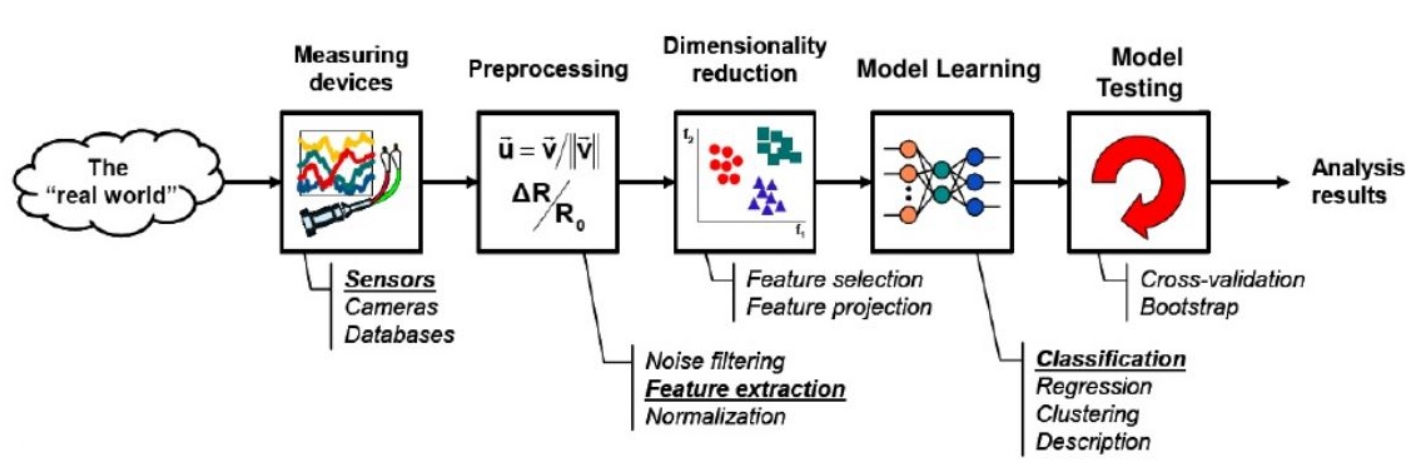
\includegraphics[width=\textwidth]{../img/Learning_process}
      \caption{Learning process in detail}
\end{figure}

\newpage

So, as can be observed in the image above, the learning process
in real-world applications where some kind of machine learning is
used is actually quite complex and it is also necessary to understand
how to perform each step of the pipeline shown below in order to build
an actually working machine learning model:

\begin{enumerate}
      \item \emph{\textbf{Data Source}}: This is the actual place where
            all data are generated. Normally this place is represented
            by the real world itself.
      \item \emph{\textbf{Data Collecting}}: This is the process by which
            all data are collected from the data source mentioned in
            point 1 by using different devices, such as
            \underline{sensors}, cameras, and databases.
      \item \emph{\textbf{Data Preprocessing}}: This is a process that
            depends on the type of the problem which is being addressed.
            Normally this process consists in some noise filtering, if the
            data are images or sensor signals, in normalization,
            if the data are seen as vectors, or in the
            so-called \emph{feature extraction}, which is achieved by
            transforming the data into a set of vectors containing relevant
            information.
      \item \emph{\textbf{Dimensionality Reduction(Optional)}}: Sometimes
            the features from the previous step are not used directly to
            produce a model, but are carefully selected to extract
            the most relevant part through the process called \emph{feature selection}.
      \item \emph{\textbf{Model Learning}}: This is the core step of the
            machine learning process in which, by applying a particular
            \emph{learning algorithm}, the actual \emph{model}
            is generated. The actual type of algorithm that will be
            applied depends on the particular nature of the problem being
            solved, such as classification, regression, clustering,
            description, and many others.
      \item \emph{\textbf{Model Testing}}: Once the model has been
            generated through a particular learning algorithm, a
            particular model testing protocol is applied to validate
            the accuracy of the generated model.
\end{enumerate}

It is also important to mention that another element that adds complexity
to the design of machine learning models is the choice of a particular
algorithm to use. This is because of the fact that there is a huge number
of machine learning algorithms that could be used. Fortunately, there is
always a guide that helps in making the right decision, that is the
particular nature of the problem to be solved.

At this point, given the general machine learning pipeline described
above, it is time to dive into the first most important element of
the process which is \emph{data}. The first
problem to solve is the fact that the concept of data is quite abstract,
but the concrete data that are used in real-world applications can be
extremely different form each other. For this reason, it is necessary to
define a general procedure that will allow representing data
independently of their actual structure. The answer to this problem is
called \emph{feature extraction}: that is the process by which each
\emph{example} in the \emph{training set} is associated with a data
structure, which is normally a simple vector of numbers with cardinality
n, that \emph{represents} the relevant information about the example and
indicates the \emph{actual form} that is seen by the algorithms. Each
such vector takes the name of \emph{feature vector}.

\newpage

One way of extracting these features is to consider them as
\emph{questions that can be asked} about the example, like for instance
in the image below with the fruits:

\vspace{5mm}

\begin{figure}[h]
      \centering
      \begin{subfigure}{0.40\textwidth}
            \centering
            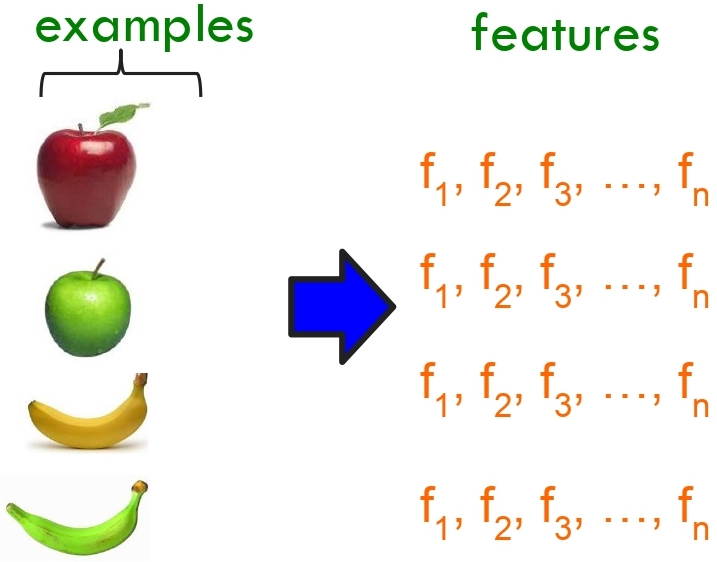
\includegraphics[width=\textwidth]{../img/Features_1}
      \end{subfigure}
      \hfill
      \begin{subfigure}{0.50\textwidth}
            \centering
            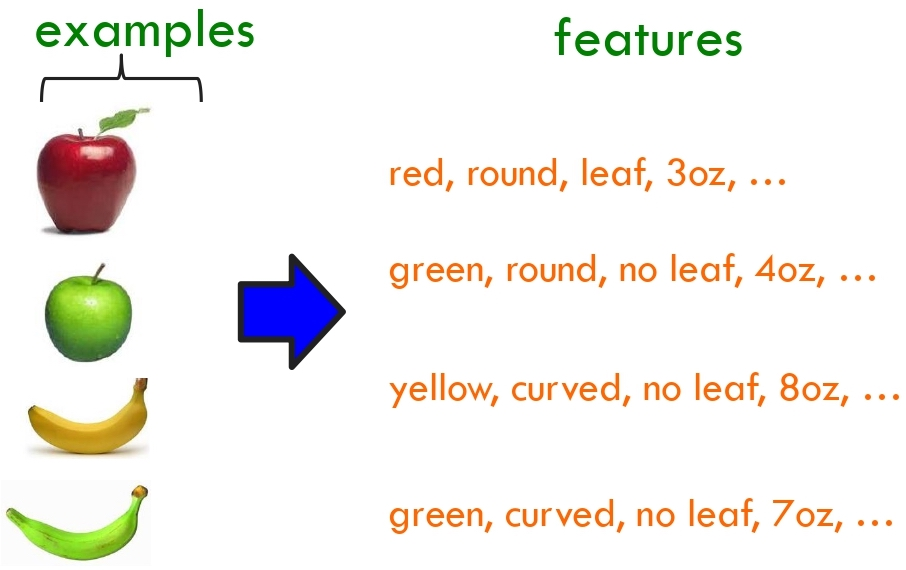
\includegraphics[width=\textwidth]{../img/Features_2}
      \end{subfigure}
      \caption{Example of features}
\end{figure}

\vspace{5mm}

Therefore, the final result of the feature extraction process is the
actual \emph{training set}, which is a set of numerical vectors, each of
which is the same dimension as the others. Unfortunately, there is a
problem with this approach, which is actually the most delicate part of
the design of the machine learning pipeline: \emph{how} are these
features chosen? There are actually many answers to this question and
the best answer should be the one that will ideally produce a set of
features that represent as well as possible the original data without
any loss of information. Therefore, there is always a risk that, after
processing the input data,
\underline{some information associated with the real data may be lost},
which in the case could cause the machine learning algorithm to work
improperly.

\subsection{Machine Learning Methods}

Now it is time to talk about different families of machine learning
methods to add a deeper understanding to what has been briefly
described in the overview subsection of these notes.

\subsubsection{Supervised Learning}

The first big family of machine learning methods is the so-called
\emph{Supervised Learning}. All methods associated with this family
have access to the data \emph{and} some annotations that are
associated with these data. These annotations are also called
\emph{labels}. Therefore, the training set, that is the input to the
learning algorithm, in these cases consists of a set of pairs, each of
which consists of an \emph{example}(in the form of a
\emph{feature vector}) and its relative \emph{label}. For this reason,
all the pairs in the training set are called \emph{labeled examples}.
Then this set of labeled examples is processed by the learning
algorithm to build a model, also called a predictor, that will be used
on new data, which have not been seen during the training phase, to
produce labels associated with these data. It is necessary to note that
all labels generated by the model will belong to the set of the
labels that have been learned from the training set. All this process
can be observed in the images below:

\newpage
% FIXME: resize the images below 

\begin{figure}[h]
      \centering
      \begin{subfigure}{0.45\textwidth}
            \centering
            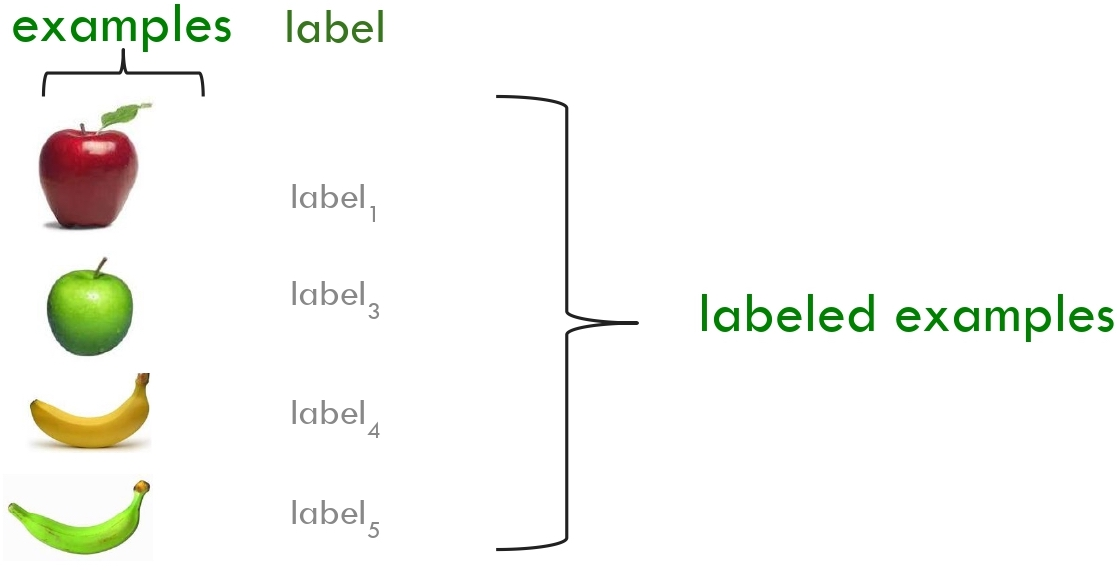
\includegraphics[width=\textwidth]{../img/Labeled_examples}
            \caption{Training Set}
      \end{subfigure}
      \hfill
      \begin{subfigure}{0.45\textwidth}
            \centering
            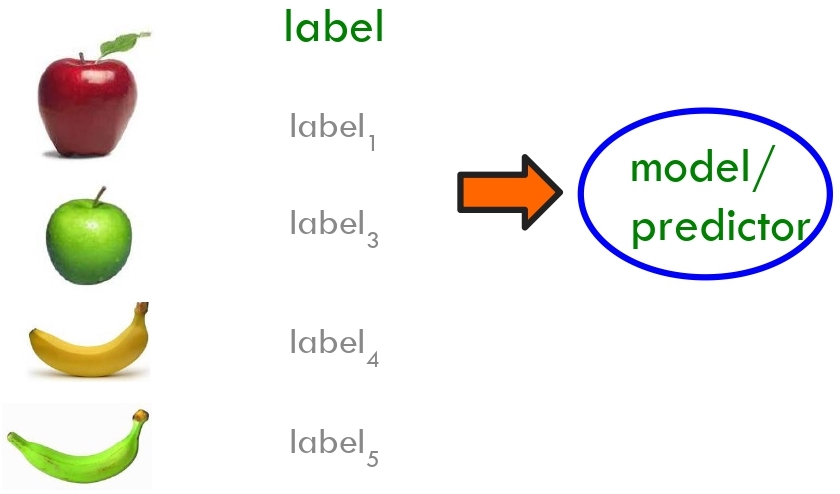
\includegraphics[width=\textwidth, height=0.55\textwidth]{../img/Supervised_training}
            \caption{Model Training}
      \end{subfigure}
      \hfill
      \begin{subfigure}{0.45\textwidth}
            \centering
            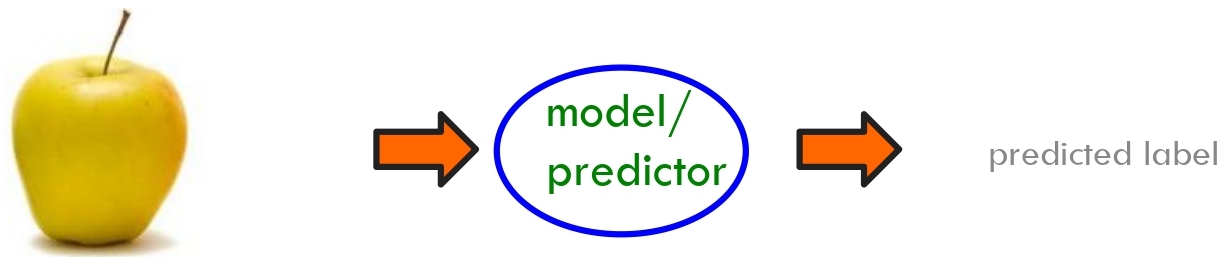
\includegraphics[width=\textwidth]{../img/Supervised_testing}
            \caption{Model Testing}
      \end{subfigure}
\end{figure}

\vspace{5mm}

At this point, it is possible to introduce some major machine learning
tasks that use the supervised learning structure defined above:

\begin{itemize}
      \item \emph{\textbf{Classification}}: Given a training set
            $\mathcal{T}=\{(x_1,y_1),...,(x_m,y_m)\}$ where
            $m$ is the total number of pairs of labeled examples,
            the task is to learn a function $f$, defined as
            $f : \mathbb{R}^d \rightarrow \{1,2,...,k\}$ where $d$
            is the dimension of the input space and $k$ is the
            \underline{finite} number of labels, to predict the label
            $y$ given the input $x$. So the dimension of the $x$
            component(feature vector) in the pairs of labeled examples
            and as input to the function $f$ is determined by the value
            of $d$, as can be observed in the examples below:

            \vspace{5mm}

            \begin{figure}[h]
                  \centering
                  \begin{subfigure}{0.52\textwidth}
                        \centering
                        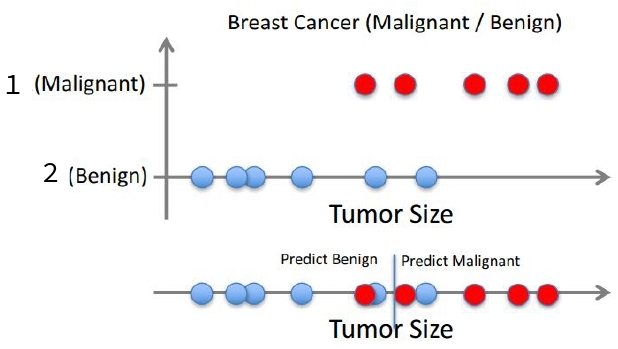
\includegraphics[width=\textwidth]{../img/Classification_1}
                        \caption{$x$ is one-dimensional($d=1$)}
                  \end{subfigure}
                  \hfill
                  \begin{subfigure}{0.38\textwidth}
                        \centering
                        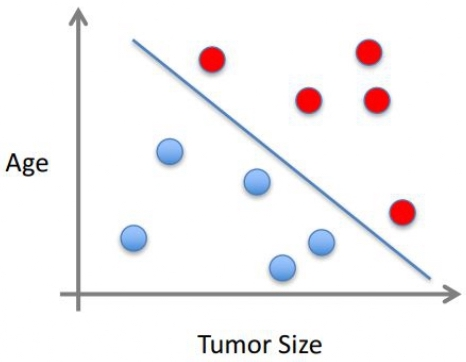
\includegraphics[width=\textwidth]{../img/Classification_2}
                        \caption{$x$ is multidimensional($d=2$)}
                  \end{subfigure}
            \end{figure}

            \vspace{5mm}

            This classification framework of supervised learning is of
            course extremely general and can be instantiated for
            several problems, such as Face Recognition, Character
            Recognition, Spam Detection, Medical Diagnosis, Biometrics
            and many others.

            \newpage

      \item \emph{\textbf{Regression}}: Given a
            training set $\mathcal{T}=\{(x_1,y_1),...,(x_m,y_m)\}$ where
            $m$ is the total number of pairs of labeled examples,
            the task is to learn a function $f$, defined as
            $f : \mathbb{R}^d \rightarrow \mathbb{R}$ where $d$
            is the dimension of the input space, to predict the label
            $y$ given the input $x$. As with Classification, the
            dimension of the $x$ component(feature vector) in the pairs
            of labeled examples and as input to the function $f$ is
            determined by the value of $d$. However, the big difference
            between Classification and Regression consists in the fact
            that all labels produced by the computed regression function
            are real-valued, so the set of all possible labels is
            \underline{not finite} by definition(i.e.\ it is
            \underline{continuous}). An example of regression is the
            following:

            \vspace{5mm}

            \begin{figure}[h]
                  \centering
                  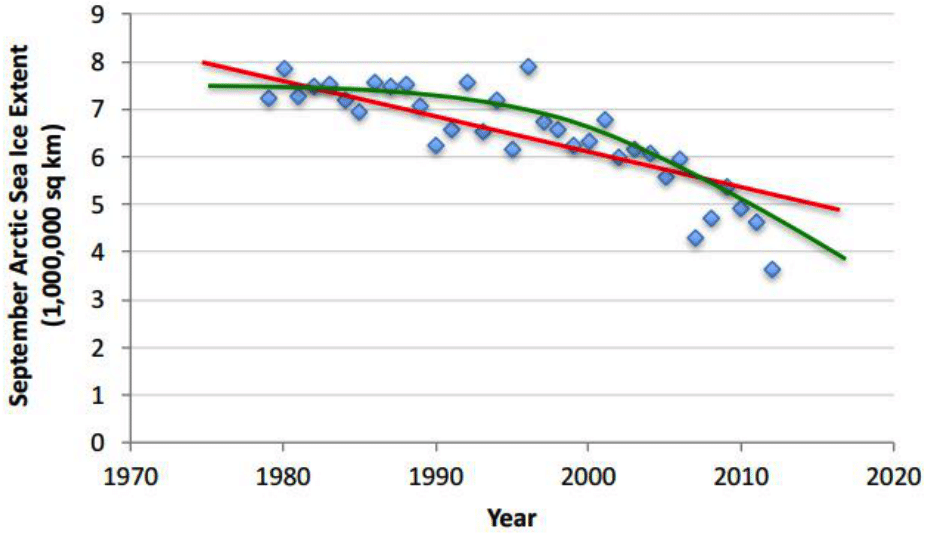
\includegraphics[width=0.7\textwidth]{../img/Regression_example}
                  \caption{Example of Regression}
            \end{figure}

            \vspace{5mm}

            As with Classification, this regression framework of
            supervised learning is of course extremely general
            and can be instantiated for several problems, such as
            Stock Value Prediction in Finance, Epidemiology, Car/Plane
            Navigation, Weather Forecasting in the area of Temporal
            Trends and many others.

      \item \emph{\textbf{Ranking}}: This is another supervised learning
            task in which all the labels in the training set and the ones
            generated by the computed ranking model are \emph{ranks},
            which are values indicating the sorting position/relevance
            of the elements. An example of ranking is search query
            evaluation in web browsers where, given a query and a set of
            web pages, a ranking is computed according to the ranks of
            the web pages, with the most relevant web sites appearing at
            the top. As with the previous two tasks, this ranking
            framework is extremely general and can be instantiated for
            several problems, such as User Preference(e.g.\ Netflix
            "My List" for movie queue ranking), Image Retrieval, Flight
            Search, Search in general and many others.
\end{itemize}

\newpage

\subsubsection{Unsupervised Learning}

The second big family of machine learning methods is the so-called
\emph{Unsupervised Learning}. As with supervised learning,
all methods associated with this family have access to the data
\emph{but} there are \emph{no} annotations associated with these data.
Therefore, the training set in this case consists only of a set
of \emph{examples}(always in the form of \emph{feature vectors})
without any associated labels. Then this set of examples is processed
by the learning algorithm to build a model consisting of a
\emph{hidden structure} behind the input data.

At this point, it is possible to introduce some major machine learning
tasks that use the unsupervised learning structure:

\begin{itemize}
      \item \emph{\textbf{Clustering}}: Given a training set
            $\mathcal{T}=\{x_1,...,x_m\}$ where m is the total number
            of examples, the task is to output a hidden structure
            behind the input data. In this particular case the
            discovered structure is represented by the so-called
            \emph{clusters}, which are perfectly illustrated in the
            following image:

            \vspace{5mm}

            \begin{figure}[h]
                  \centering
                  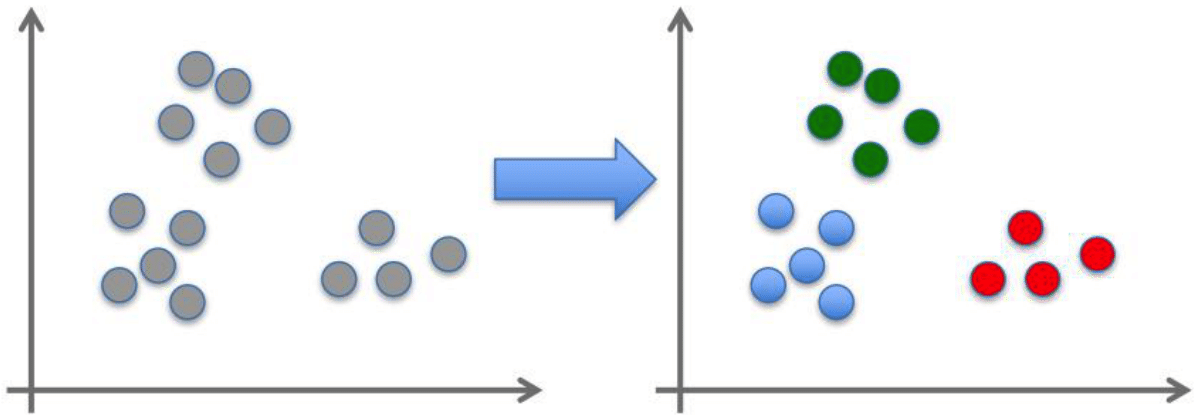
\includegraphics[width=0.8\textwidth]{../img/Clustering_example}
                  \caption{Example of Clustering}
            \end{figure}

            \vspace{5mm}

            This clustering framework of unsupervised learning is of
            course extremely general and can be instantiated for
            several problems, such as Social Network Analysis, Genomics,
            Image Segmentation and many others.

      \item \emph{\textbf{Anomaly Detection}}: This is another
            unsupervised learning task in which the training set consists
            of events or objects and the task consists in detecting those
            events or objects that are unusual or atypical.

            This anomaly detection framework of unsupervised learning
            is of course extremely general and can be instantiated for
            several problems, such as Credit Card Fraud Detection,
            Video Surveillance and many others.

            \newpage

      \item \emph{\textbf{Dimensionality Reduction}}: This is another
            unsupervised learning task in which the training set consists
            of data characterized by a certain number of dimensions
            (i.e.\ variables) and the task is to reduce these dimensions
            in order to get a set of data characterized by a reduced
            number of variables while preserving the most important
            relationships between the data as they were in the initial
            set. This particular task can be observed in the following
            image:

            \vspace{5mm}

            \begin{figure}[h]
                  \centering
                  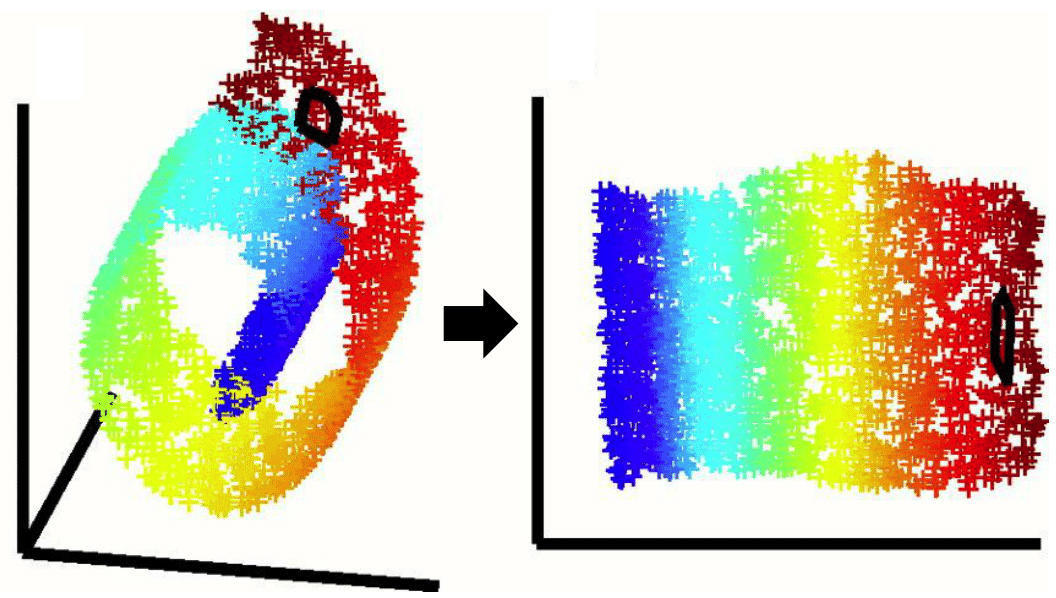
\includegraphics[width=0.45\textwidth]{../img/Dim_reduction_example}
                  \caption{Example of Dimensionality Reduction}
            \end{figure}

            \vspace{5mm}

            This dimensionality reduction framework of unsupervised
            learning is of course extremely general and can be
            instantiated for several problems, such as Output Inspection
            in the case of a classification algorithm and many others.
\end{itemize}

\subsubsection{Reinforcement Learning}

The third big family of machine learning methods is the so-called
\emph{Reinforcement Learning}. The big difference between this
family and the previous two consists in the fact that there is no
training set in reinforcement learning but there is only a numerical
performance score as its guidance. Therefore, in this case there is a
totally different learning scheme, which is based on the following idea:
an \emph{agent} learns from an \emph{environment} by interacting with
it through some \emph{actions} that make it receive \emph{rewards}
and make it modify its current \emph{state}. This idea is clearly
illustrated in the following image:

\vspace{2mm}

\begin{figure}[h]
      \centering
      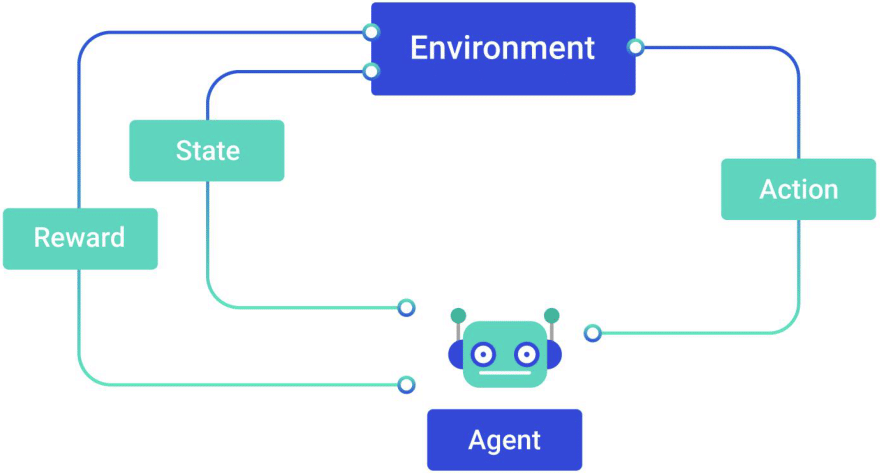
\includegraphics[width=0.5\textwidth]{../img/Reinforcement_learning}
      \caption{Reinforcement Learning Scheme}
\end{figure}

\vspace{5mm}

\newpage

It immediately becomes clear that this learning scheme is highly
\emph{interactive} because the agent, in order to learn some useful
information, continuously completes \emph{sequences of states/examples}
and gets \emph{rewards} after completing those sequences. In this way,
based on the values of the rewards, the agent learns to predict the
\emph{action} to take for each individual state/example in order to
achieve its final goal, which is an optimal, or nearly-optimal, way to
maximize the amount of gained rewards. An example of a sequence evaluation
is illustrated in the following image:

\vspace{5mm}

\begin{figure}[h]
      \centering
      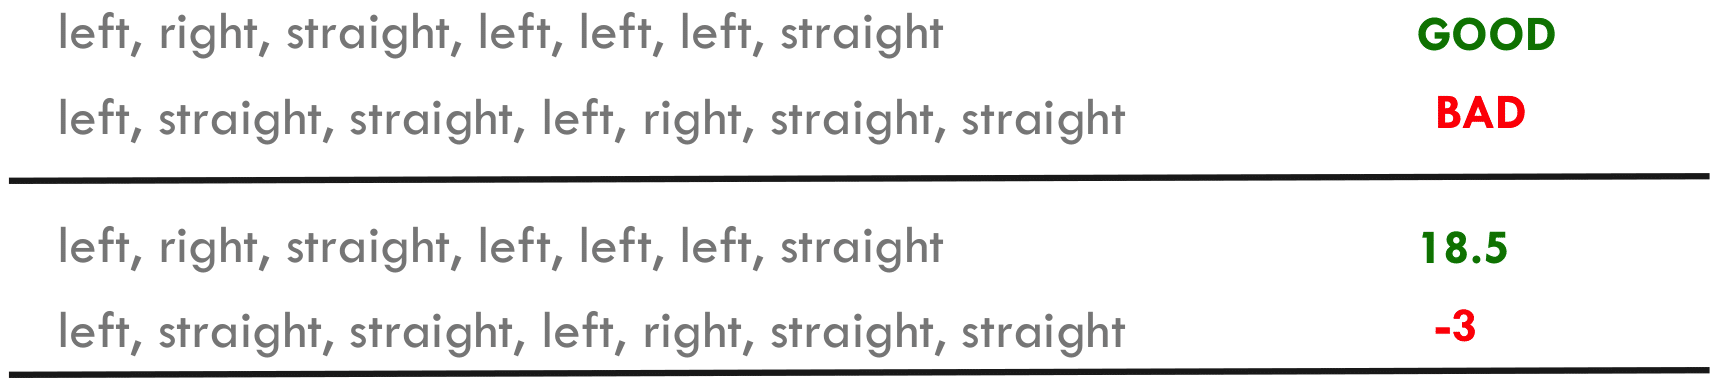
\includegraphics[width=0.8\textwidth]{../img/Sequence_example}
      \caption{Example of a sequence evaluation}
\end{figure}

\vspace{5mm}

Some famous examples of the application of reinforcement learning are
for instance the Backgammon and Go board games and the computer game
Atari Breakout, in which you try to learn winning sequences.

\subsubsection{Other Learning Variations}

Besides the three largest families of machine learning methods,
there are other families that will not be covered in these notes.
However, it is always useful to mention \emph{some} of them because
of their usage in different areas:

\begin{itemize}
      \item \emph{\textbf{Semi-supervised Learning}}: This is a family
            of hybrid machine learning methods that involve small
            datasets of labeled examples(supervised learning) and large
            datasets of examples that don't contain any
            labels(unsupervised learning).

            \vspace{5mm}

            \begin{figure}[h]
                  \centering
                  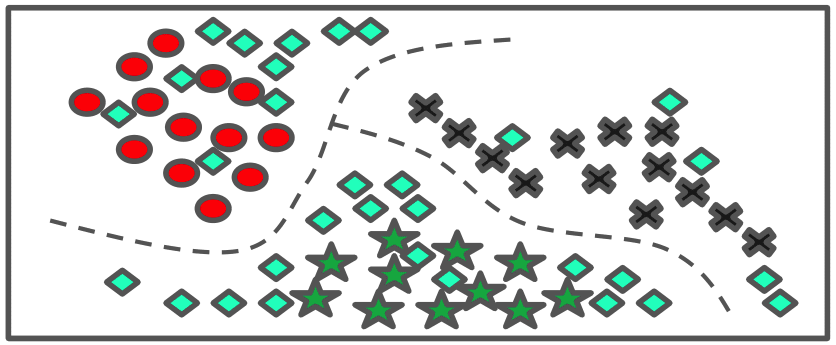
\includegraphics[width=0.6\textwidth]{../img/Semi_supervised_learning}
                  \caption{Example of Semi-supervised Learning}
            \end{figure}

            \vspace{5mm}

            \newpage

      \item \emph{\textbf{Active Learning}}: This is a family of machine
            learning methods that are characterized by an incremental
            learning scheme and by some human supervision(some useful
            feedback) which is involved only in the case of the most
            difficult examples.

            \vspace{5mm}

            \begin{figure}[h]
                  \centering
                  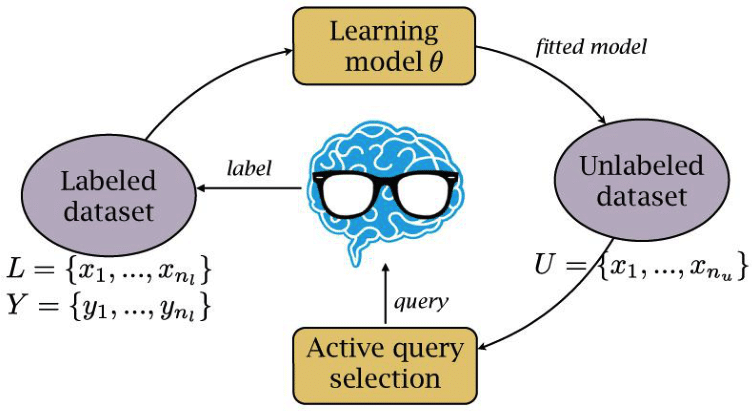
\includegraphics[width=0.55\textwidth]{../img/Active_learning}
                  \caption{Example of Active Learning}
            \end{figure}

            \vspace{5mm}
\end{itemize}

\noindent Some learning variations also derive from \emph{how} the data
are retrieved:

\begin{itemize}
      \item \emph{\textbf{Online Learning}}: There is a continuous
            process during which the incoming data are immediately
            used to update the model.

      \item \emph{\textbf{Offline Learning}}: The data, such as training
            sets, are available offline and are used to train a model
            that will then be used on new unknown data.
\end{itemize}

\noindent Other learning variations also derive from the \emph{type} of
a model:

\begin{itemize}
      \item \emph{\textbf{Generative vs Discriminative Learning}}:
            These two different types will be covered in the
            particular case of supervised learning later in these notes.
      \item \emph{\textbf{Parametric vs Non-parametric Learning}}:
            Some models may or may not contain some parameters that
            are learned during the training phase.
\end{itemize}

\subsection{Intro to Data Generating Distributions}

Now it is time to talk more deeply about one of the most relevant
and critical elements of machine learning, that is \emph{features}
and their \emph{generation}. As mentioned previously, the training
set is made of examples(labeled in the case of supervised learning)
that are represented in the form of features and then the model,
that is generated during the training phase, makes predictions
\emph{\textbf{based on these features}}. The testing set is also made of
examples that are represented in the form of features, but in this
case, no answers are provided, since the answers will be generated by
the model, which will process the features of each example to produce
the predictions(labels in the case of supervised learning).

\newpage

The natural question that arises from this summary is how the training
and testing sets should be generated. The natural answer to this
question is that the same feature extraction algorithm should be applied
to generate both the training and testing sets, but this is not enough.
The fact is that the result of a prediction will strongly depend on the
features that have been seen, so the examples in the testing set should
contain features that are \emph{similar} to some features in some
examples in the training set. This is an intuition that has to be
formalized and satisfied in order to be able to
\emph{\textbf{generalize from the training set}}. So the implicit
assumption here is that the examples in the testing set are
\emph{in some way similar} to the examples in the training set.
This is not always the case, but sometimes it will be necessary
to assume that it is.

At this point, it is necessary to formalize the intuition described
above and this can be achieved by modeling the similarity between
the training and testing sets through a \emph{probabilistic model}
of learning. This probabilistic modeling implies
\emph{\textbf{the most important assumption of machine learning}},
that is the fact that \textbf{it is possible to learn} because it is
\textbf{assumed} that \textbf{both} the training
\textbf{and} testing sets are generated by the \textbf{same} underlying
probability distribution, which is \textbf{unknown} and called in
this context \textbf{Data Generating Distribution(DGD)}.
So, thanks to this assumption, it is possible to build systems that
can generalize between the training and testing sets by starting to
consider the different features of the examples in the training
and testing sets in terms of probability, as can be observed in the
following image:

\vspace{5mm}

\begin{figure}[h]
      \centering
      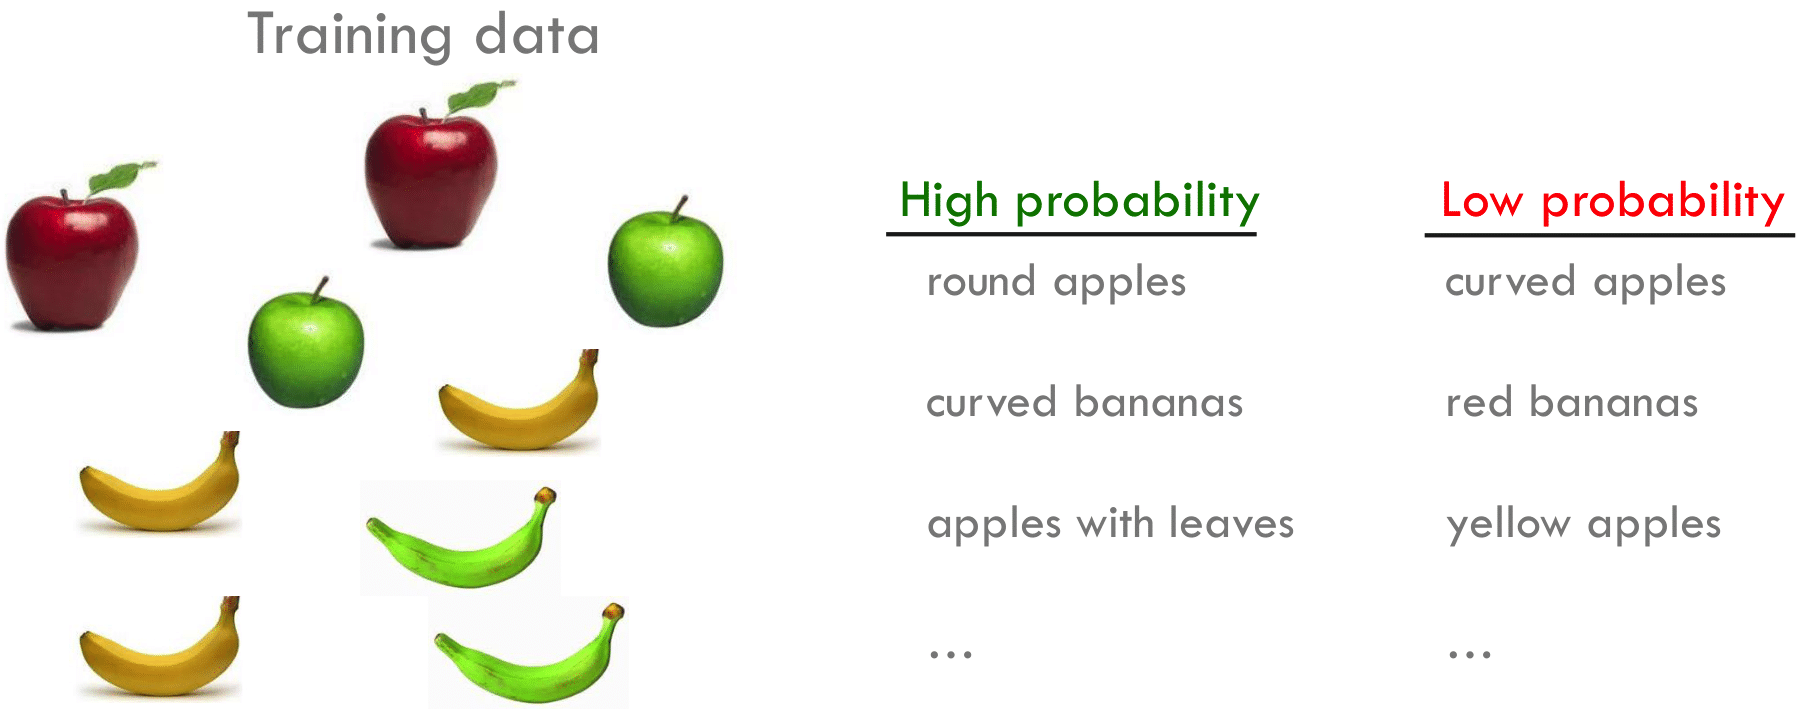
\includegraphics[width=0.6\textwidth]{../img/Testing_set_prob}
      \caption{Example of probability values}
\end{figure}

\vspace{5mm}

In order to start getting familiar with the concept of data generating
distribution it could be useful to observe the following image, which
represents a data generating distribution with different
\emph{likelihood values of sampling}, for every fruit category,
in terms of different amounts of fruits:

\newpage

\begin{figure}[h]
      \centering
      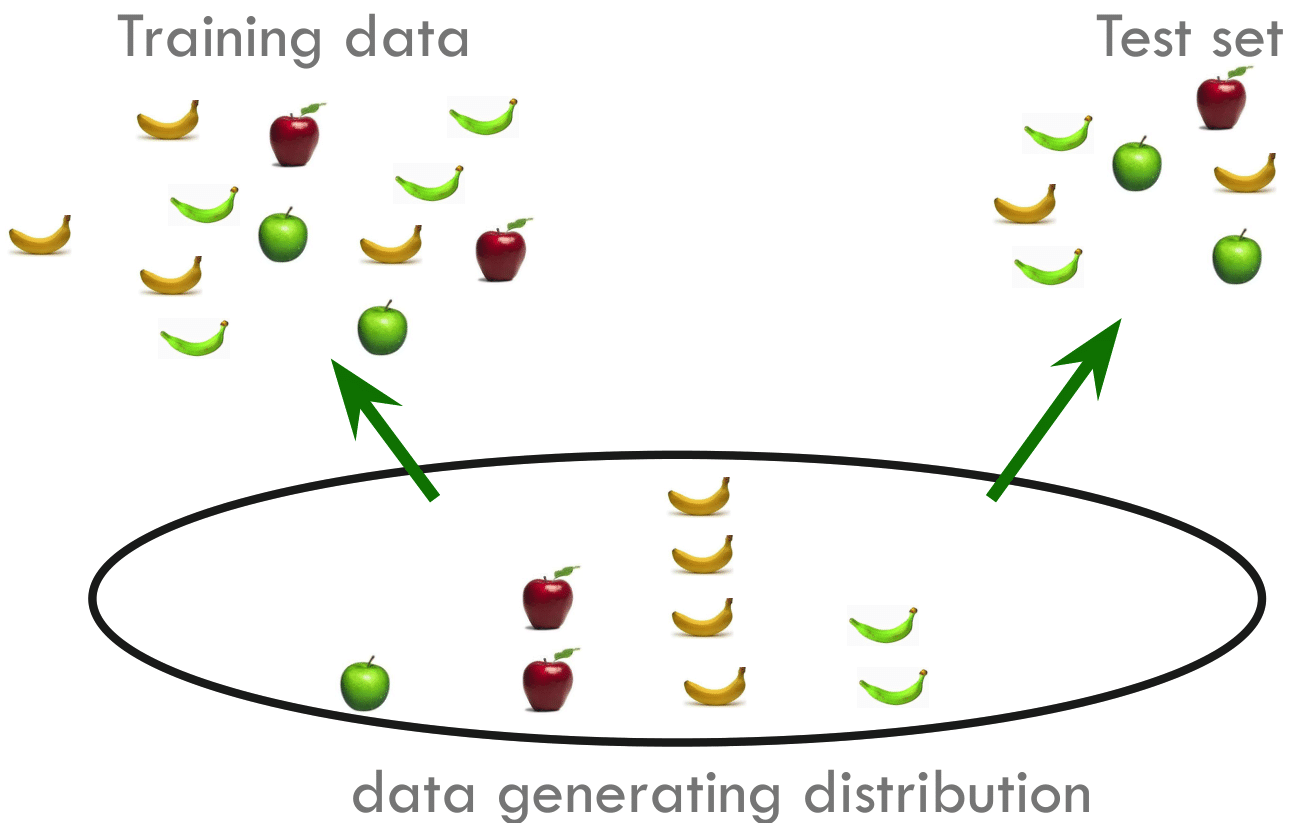
\includegraphics[width=0.6\textwidth]{../img/DGD_example}
      \caption{Example of a DGD}
\end{figure}

\vspace{5mm}

It is also extremely useful to observe some counterexamples that
clarify even more the importance of the fact that both the training
and testing sets must be generated by the same probability distribution:

\vspace{5mm}

\begin{figure}[h]
      \begin{subfigure}{0.45\textwidth}
            \centering
            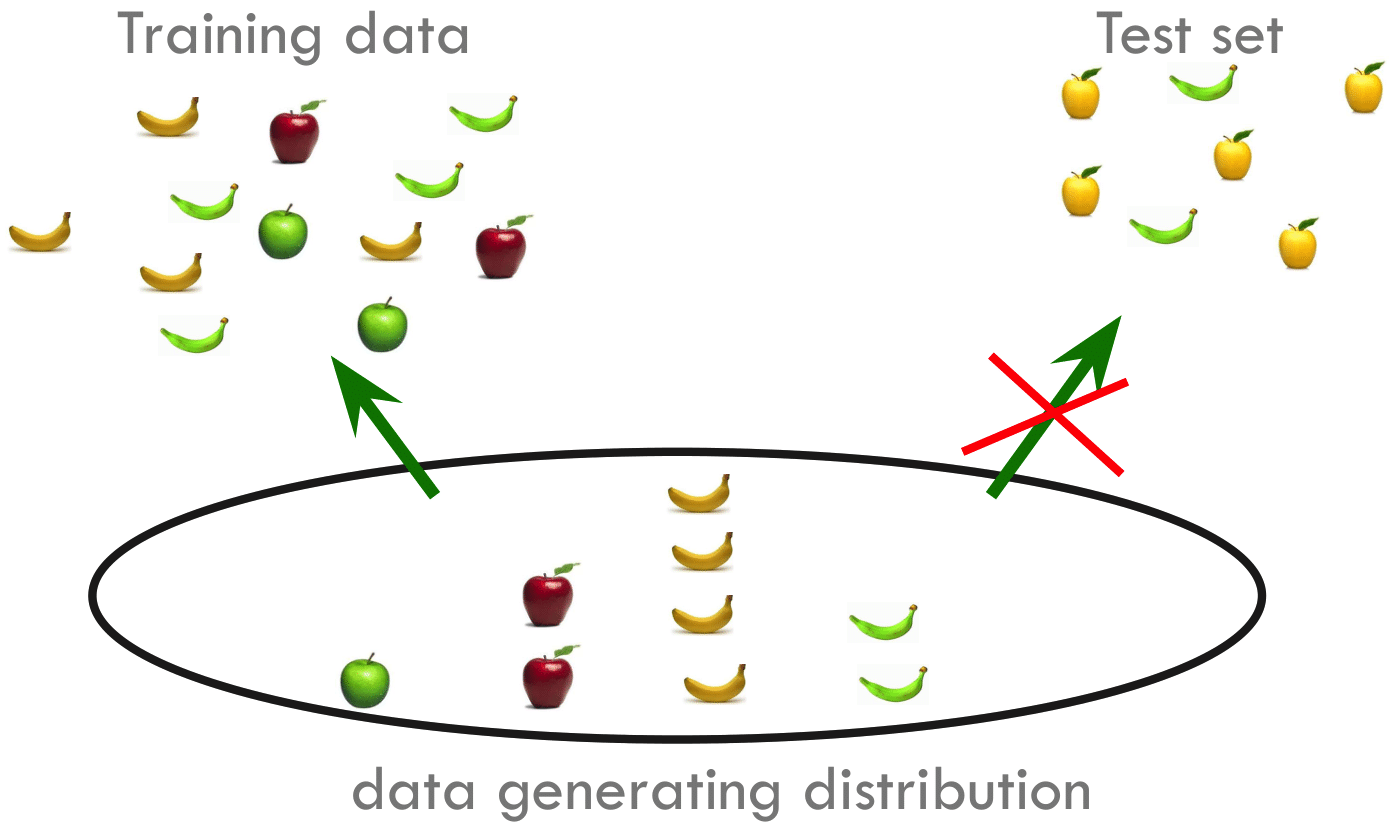
\includegraphics[width=\textwidth]{../img/DGD_counterexample_1}
            \caption{Testing Set with new fruits}
      \end{subfigure}
      \hfill
      \begin{subfigure}{0.45\textwidth}
            \centering
            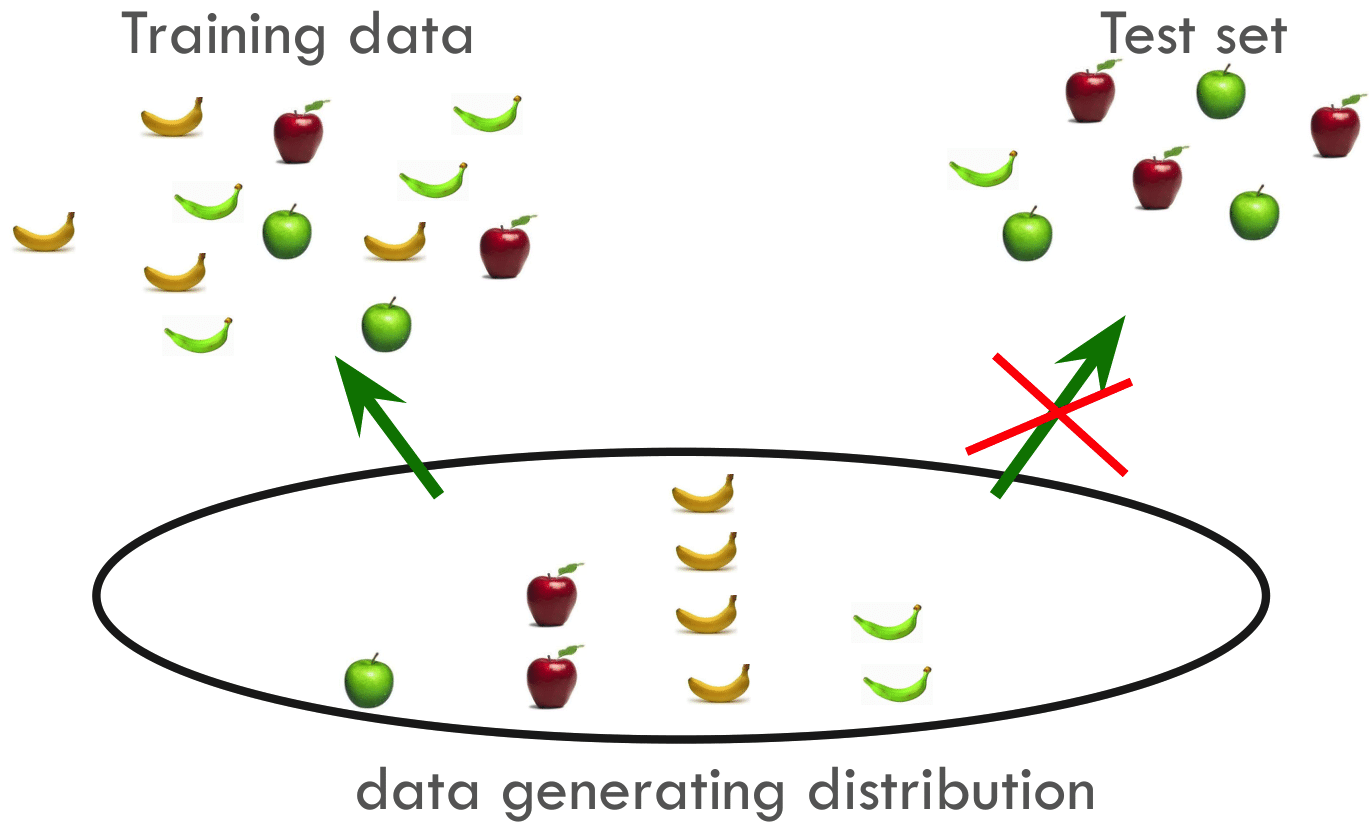
\includegraphics[width=\textwidth]{../img/DGD_counterexample_2}
            \caption{Testing Set without bananas}
      \end{subfigure}
      \caption{Training and Testing Sets generated by different DGDs}
\end{figure}